\begin{figure}[!h]
\centering
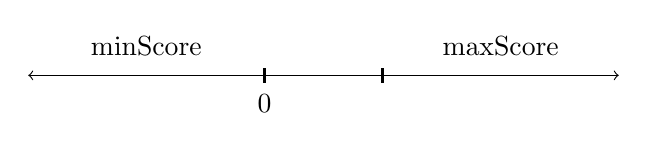
\begin{tikzpicture}[]
    \draw[<-] (0,0) -- (1.5,0);
    \draw[{[-|}] (1.5,0) node[label=above:{minScore}] {} -- (3,0) node[label=below:{0}] {};
    \draw[{|-|}] (3,0) node[label=below:{}] {} -- (4.5,0) node[label=below:{}] {};
    \draw[{|-]}] (4.5,0) node[label=below:{}] {} -- (6,0) node[label=above:{maxScore}] {};
    \draw[->] (6,0) node[label=below:{}] {} -- (7.5,0) node[label=below:{}] {};
\end{tikzpicture}
\caption{Rango de puntajes Needleman-Wunsch}
Fuente: Elaboracion propia.
\label{intervalNW}
\end{figure}
